\section{Field}
The Field consists of several components; the Track, Pickup and Launch zones, three Obstacles, the Target and the Sprint. A general description of each component follows below. Models and dimensioned drawings of each of the Field’s components can be found in the {\col\href{https://mercury.okstate.edu/content/mercury-challenge}{2019 Track Pack}.

\begin{figure}[H]
	\centering
%	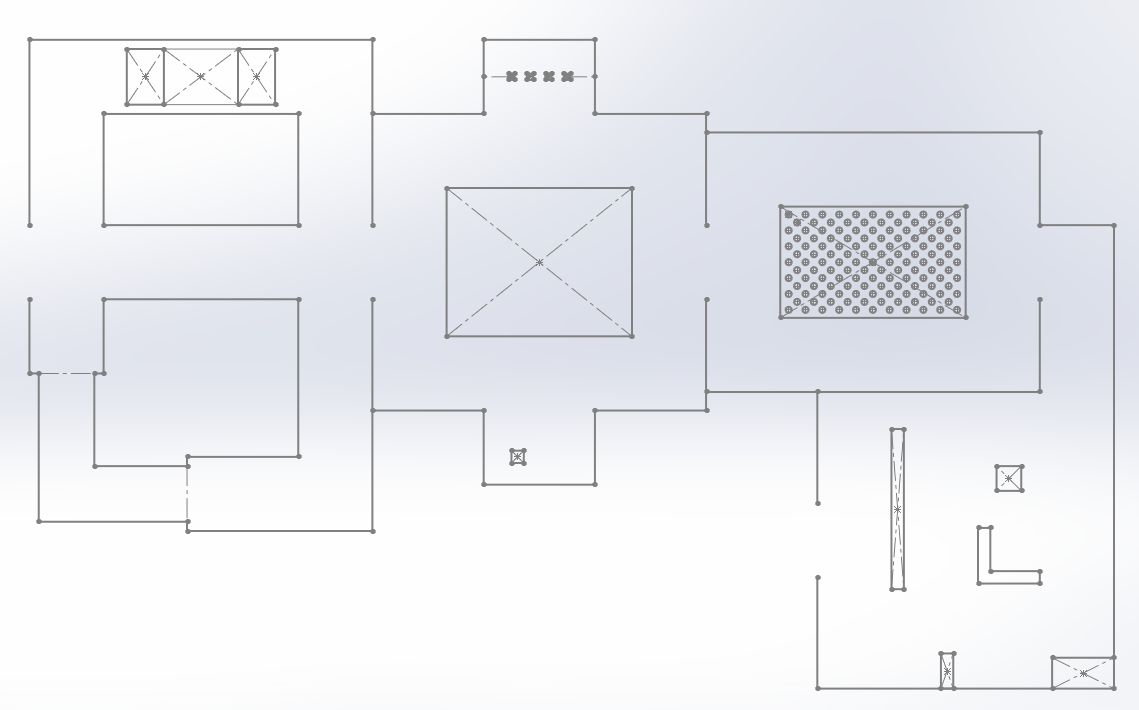
\includegraphics[scale=.5]{images/track_overview_wlabels.jpg}
	\caption{Field Overview}
	\label{fig:field} 
\end{figure}

\subsection{Track}
The Track is defined as a 24 inch wide path that is bounded on either side by 3 inch high walls. The walls used at the Competition will be constructed from foam board of the type that is easily obtainable from craft stores; 1/8 inch thick with a matte, white paper surface. The track floor will be short pile carpet.

\subsection{Pickup Zone}
This area is defined as a 24 inch square, dead end section of track that will hold the Payload for pickup by the robot. The team is allowed to choose the placement of the Payload within the Pickup Zone prior to the start of a run. The robot and Payload are the only objects permitted in the Pickup Zone at any time during a run. 

\subsection{Obstacles}
Although the 2019 Competition Track does not include any paths that bypass the Obstacles, a team may choose to bypass any or all of the obstacles during a run. See section \ref{bypass} for details.
\subsubsection{Tunnel}
The Tunnel is an L-shaped wooden structure with openings on either end that are 12 inches high by 18 inches wide. The interior is dark. This Obstacle tests the maneuverability of the robot in a confined space with limited visibility.

\subsubsection{Bridge}
The Bridge is 24 inches wide with a smooth wooden surface and no guard walls. The climb is 30 degrees with 12 inch rise, followed by a 24 inch span and a 30 degree descent. This Obstacle tests the robot’s ability to move in a controlled manner on an inclined surface.

\subsection{Launch Zone}
The Launch Zone is a 2 foot wide opening in the Track wall from which the Robot will Launch the Payload. While it is permissible for the for part of the robot to extend over or through this opening, a penalty will be incurred if the main body of the Robot crosses the boundary determined by the walls at either side. 

\subsection{Target}
The Target is a freestanding object that the Payload is launched to in order to score points. It will be placed in the area where the Track forms a loop. Points are awarded according to which of the Target’s three openings the Payload falls into.

\subsection{Sprint}
The final section of the Track is a 40 foot long straight run timed by infrared tripwires at both ends. This portion of the Field will test the speed and straight line control of the robot. The points earned in this section will be a multiplier for the total points acquired in a run by the robot.